\documentclass[a4paper,11pt,oneside]{report}
\usepackage[pdftex]{graphicx}
\usepackage[utf8x]{inputenc}
\usepackage[spanish]{babel}
\usepackage{fancyhdr}
\usepackage[Bjornstrup]{fncychap}
\usepackage{tabularx}
\usepackage{hyperref}
\usepackage{eurosym}
\usepackage{longtable}
\usepackage[table]{xcolor}
\usepackage{verbatim}
% \usepackage[usenames,dvipsnames]{color}
% \usepackage{colortbl}
% \usepackage[caption=false]{subfig}
% \usepackage{float}
% \usepackage{pdflscape}

\setlength{\headheight}{25pt}
\setlength{\parskip}{6pt}

% Margenes 1cm mas pequennos
% \addtolength{\oddsidemargin}{-1cm}
% \addtolength{\evensidemargin}{-1cm}
% \addtolength{\textwidth}{2cm}
% \addtolength{\voffset}{-1cm}
% \addtolength{\textheight}{2cm}

\lhead{
\includegraphics[height=20pt]{logo-umbrella.png}}
\chead{}
\rhead{\nouppercase{\leftmark}}

\hypersetup{
colorlinks,
citecolor=black,
filecolor=black,
linkcolor=black,
urlcolor=black
}

 % La que hay que liar para que las cabeceras de los capitulos
 % no tiren media pagina a la basura...

\makeatletter
\def\@makechapterhead#1{{
\parindent \z@ \raggedright \normalfont
\ifnum \c@secnumdepth >\m@ne
	\if@mainmatter
		\DOCH
	\fi
\fi
\interlinepenalty\@M
\if@mainmatter
	\DOTI{#1}
\else
	\DOTIS{#1}
\fi
}}

\def\@makeschapterhead#1{{
\parindent \z@ \raggedright
\normalfont
\interlinepenalty\@M
\DOTIS{#1}
}}
\makeatother

\begin{document}

\renewcommand\listtablename{Índice de tablas}
\renewcommand\tablename{Tabla}

\pagestyle{plain}

%%%% Title Page %%%%%

\pagenumbering{alph}

\begin{titlepage}
\begin{center}

% Logo

\includegraphics[width=0.6\textwidth]{logo-umbrella.png}\\[4cm]

% Title
{\huge \textbf{La Conquista del Mundo}}\\[0.5cm]
{\huge {Memoria del proyecto}}\\[4cm]

% Authors
\begin{minipage}{0.5\textwidth}
\large
\hspace{1cm}\textbf{\emph{Director de proyecto}}\\
Ricardo Ruedas García\\
\end{minipage}

\begin{minipage}{0.5\textwidth}
\large
\hspace{1cm}\textbf{\emph{Equipo de desarrollo}}\\
Jorge Colao Adán\\
Ángel Durán Izquierdo\\
Antonio Gómez Poblete\\
Daniel León Romero\\
Antonio Martín Menor de Santos\\
Laura Núñez Villa\\
\end{minipage}\\[2cm]

{\Large \today}
\end{center}
\end{titlepage}

%%%% end Title Page %%%%%

\clearpage
\pagenumbering{arabic}
\setcounter{page}{2}

\tableofcontents
\addcontentsline{toc}{chapter}{\contentsname}
% \listoffigures
% \listoftables

\clearpage

\pagestyle{fancy}

\chapter{Introducción}

\section{Descripción del juego}

\textit{La Conquista del Mundo} es un juego de estrategia por turnos que es
jugado sobre un tablero que representa el mapa del mundo. Este mapa está
dividido en 42 territorios.

Cada jugador comienza con un territorio y, por turnos, podrá realizar distintas
acciones como comprar nuevas unidades o territorios, o invadir territorios
enemigos. Todas estas acciones van dirigidas a alcanzar el objetivo del juego:
conquistar el mundo.

\section{Sistema distribuido}

La aplicación constituye un sistema distribuido. Los alumnos de la asignatura
formarán un total de cinco grupos. De éstos, uno de ellos se encargará del
desarrollo del servidor. El resto de grupos, entre los que se incluye éste,
realizarán independientemente clientes para este sistema.

Las comunicaciones entre las distintas aplicaciones se realizarán haciendo uso
del \textit{middleware} de comunicaciones RMI de Java. Para ello, se ha escrito
una interfaz común de clases para transmitir los datos entre los clientes y
el servidor.

\section{Visión general del documento}

% TODO

\chapter{Arquitectura}

La aplicación sigue una variación de la arquitectura de tres capas. Las capas
de presentación y dominio permanecen inalteradas. Sin embargo, esta aplicación
no necesita de almacenamiento externo, sino que se obtiene esta información
directamente del servidor. Por ese motivo, la capa de persistencia ha sido
sustituida por una capa de comunicaciones.

\begin{figure}[h]
\caption{Visión general de la arquitectura}
\centering
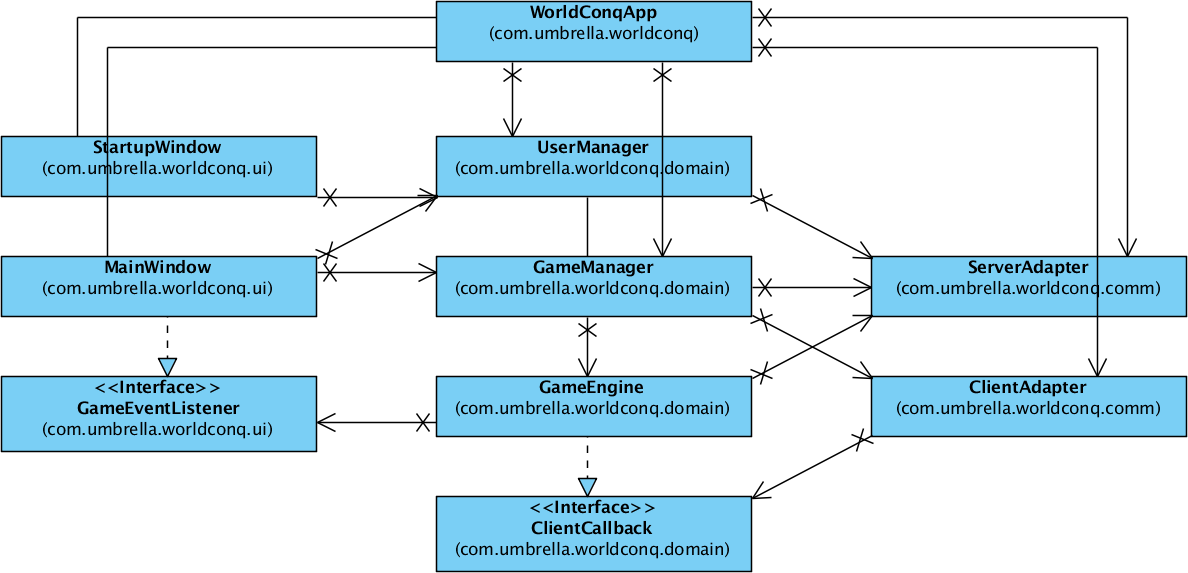
\includegraphics[scale=0.4]{img/ch02arch-overview.png}
\end{figure}

La visibilidad entre clases va de manera jerárquica, de manera que las clases
de presentación conocen a las de dominio, y las de dominio a las de
comunicaciones, pero no al revés. Para los casos en los que es necesario un
flujo de información en sentido contrario, se han creado interfaces para
desacoplar en la medida de los posible las capas inferiores.

La clase \texttt{WorldConqApp} es la única clase que no pertenece a ninguna de
las capas. Su función es la de ser el punto de entrada de la aplicación,
encargada de crear la estructura de clases, sus relaciones, y configurarlas a
partir de los parámetros de entrada.

\section{Capa de comunicaciones}

Esta capa contiene las clases \texttt{ServerAdapter} y \texttt{ClientAdapter}.
Ambas clases sirven de pasarela para los datos que fluyen entre el servidor y la
capa de dominio.

Estas clases incluyen una pequeña lógica de control. En el caso de la clase
\texttt{ServerAdapter}, ésta debe ser configurada con los datos del servidor
para así poder crear el \textit{proxy} a la interfaz remota. La ausencia de
esta configuración generará una excepción.

La clase \texttt{ClientAdapter} en cambio escucha todas las peticiones que
realiza el servidor sobre el cliente. Esta clase filtra estas peticiones de
acuerdo al juego activo en ese momento, descartando aquellas que no concuerden.

\section{Capa de dominio}

Esta capa está dividida en tres clases que se corresponden con los tres módulos
funcionales de la aplicación: gestión de usuarios, gestión de partidas, y motor
de juego.

La clase \texttt{UserManager} es la encargada de crear nuevas cuentas en la
aplicación y de mantener la información de la sesión activa. A esta clase
acceden el resto de clases para obtener la información sobre el jugador. De
manera análoga, la clase \texttt{GameManager} gestiona el listado, creación y
carga de partidas.

\begin{figure}[h]
\caption{Modelos de datos}
\centering
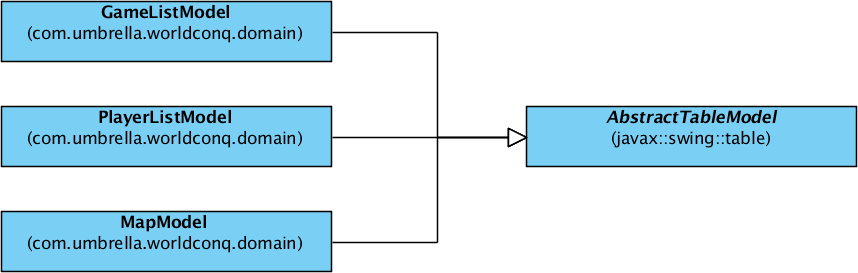
\includegraphics[scale=0.4]{img/ch02arch-models.png}
\end{figure}

Los datos de las partidas disponibles en el servidor son almacenados en objetos
de tipo \texttt{GameListModel}. Esta clase, y otras que se describen a
continuación, heredan de la clase \texttt{AbstractTableModel}. Esta clase
abstracta forma parte del \textit{framework} que proporciona Swing para
implementar el patrón arquitectónico Model-Vista-Controlador.

Hacer uso de este \textit{framework} significa que los accesos que hacen las
vistas a los modelos están definidos de antemano por una serie de interfaces.
Esto permite asociar clases disponibles en Swing con clases implementadas por el
equipo de trabajo de forma transparente.

En último lugar está el motor de juego, la clase \texttt{GameEngine}. Esta
clase se crea al comenzar a jugar a una partida e implementa toda la lógica de
dominio de una partida. Los datos con los que trabaja están almacenados en las
clases \texttt{PlayerListModel} y \texttt{MapModel}, los cuales heredan de la
clase \texttt{AbstractTableModel}, nombrada anteriormente.

\section{Capa de presentación}

En esta capa se encuentra la clase \texttt{StartupWindow}. Esta clase
representa a la primera ventana que se muestra. En ella, el usuario puede
registrar un nuevo usuario en el sistema y acceder con él.

Una vez accedido, se muestra la ventana principal, representada por la clase
\texttt{MainWindow}. Dentro de esta ventana existen dos modos de ejecución: el
modo de sala de espera y el modo partida.

\begin{figure}[h]
\caption{Vistas de datos}
\centering
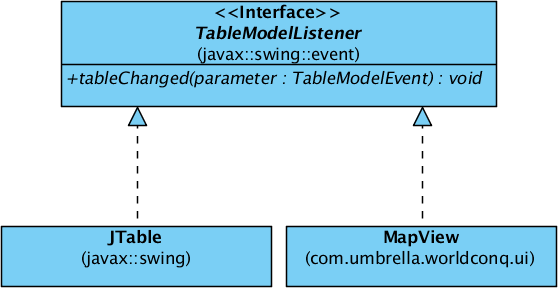
\includegraphics[scale=0.4]{img/ch02arch-views.png}
\end{figure}

En el modo de sala de espera, el usuario puede ver las partidas disponibles o
crear otras nuevas. Una vez se decida a cual jugar, la aplicación pasa a modo
partida.

La interfaz del modo partida se compone principalmente del mapa de juego. Junto
a él existen otro paneles informativos con los jugadores en la partida o una
lista con los últimos eventos.

Tanto las listas de partida como el mapa de juego implementan la interfaz
\texttt{TableModelListener}. Esto permite que estas clases puedan ser añadidas
como observadores de los cambios que sucedan en los modelos de datos.

\chapter{Desarrollo}

En este capítulo se hará un seguimiento del desarrollo completo del proyecto,
organizado por casos de uso. Para cada caso de uso, se comenzará hablando sobre
las decisiones de diseño tomadas. Un siguiente apartado tratará sobre cualquier
aspecto relevante de la implementación. Por último se mostrará un informe de
pruebas.

La documentación de este capítulo no sustituye al proyecto realizado con Visual
Paradigm, sino que destaca los aspecto más importantes para su mejor
comprensión.

\subsection{Registrarse}

\begin{figure}[ht]
\centering
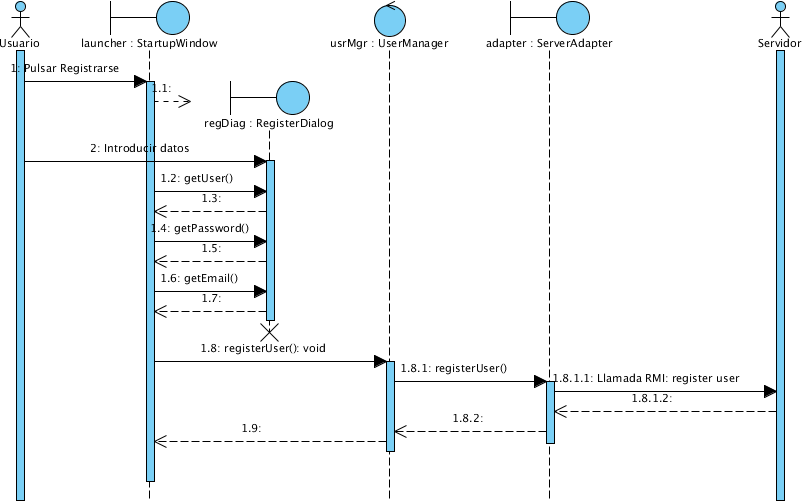
\includegraphics[scale=0.6]{img/ch03devel-register.png}
\caption{Diagrama de secuencia de ``Registrarse''}
\end{figure}

Cuando el usuario pulse el botón ``Registrarse'', se mostrará el diálogo de
registro \texttt{RegisterDialog}. Este diálogo se ejecutará de manera modal,
por lo que bloqueará el flujo de ejecución en la aplicación principal hasta que
el usuario lo complete.

A continuación, la aplicación llamará a la función correspodiente en el gestor
de usuarios para llevar a cabo el registro. Éste a su vez realizará la llamada
RMI a través del \texttt{ServerAdapter}.

Este caso de uso no provoca cambios en el estado interno del gestor de usuarios.

\subsection{Iniciar sesión}

\begin{figure}[ht]
\centering
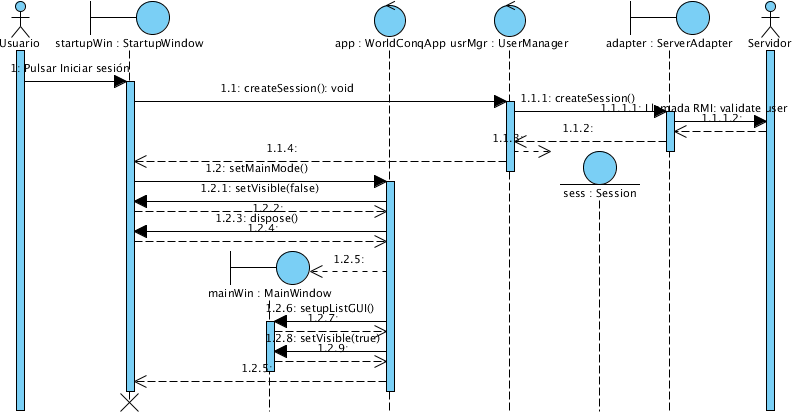
\includegraphics[scale=0.6]{img/ch03devel-login.png}
\caption{Diagrama de secuencia de ``Iniciar sesión''}
\end{figure}

Una vez que el usuario haya introducido sus credenciales, la ventana
\texttt{StartupWindow} pedirá al gestor de usuarios que inicie una nueva
sesión. El gestor de usuarios realizará la llamada RMI a través del
\texttt{ServerAdapter}.

Si los datos son correctos, el servidor devolverá un identificador de sesión.
Con este identificador y el propio nombre de usuario, el gestor de usuarios
creará un nuevo objeto de tipo \texttt{Session}.

A continuación, la ventana \texttt{StartupWindow} pedirá a la clase
\texttt{WorldConqApp} el cambio al modo principal. Al realizar este cambio, se
ocultará la ventana de inicio y se creará la nueva ventana principal
\texttt{Mainwindow}.

\subsection{Cerrar sesión}

\begin{figure}[ht]
\centering
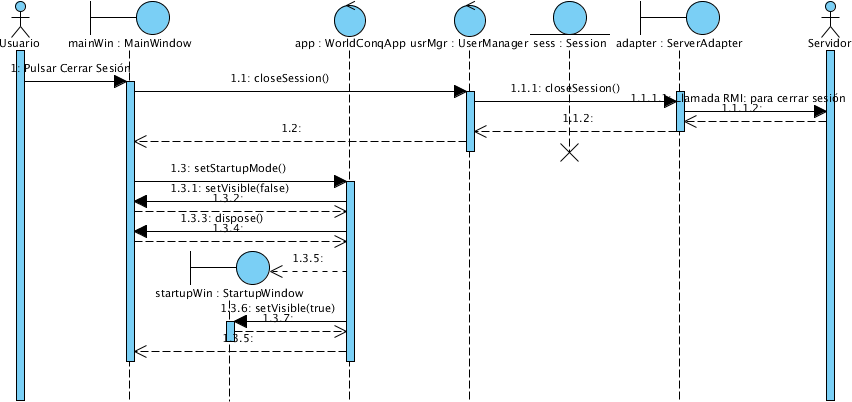
\includegraphics[scale=0.6]{img/ch03devel-logout.png}
\caption{Diagrama de secuencia de ``Cerrar sesión''}
\end{figure}

Estando en la ventana principal, el usuario puede decidir cerrar sesión en
cualquier momento. Este evento genera una llamada al gestor de usuarios. El
gestor de usuarios comunica al servidor que el usuario quiere cerrar la sesión.
Así mismo, destruirá la sesión que había hasta ahora.

A continuación se solicita a la clase \texttt{WorldConqApp} que vuelva a la
ventana de inicio realizando el paso inverso al detallado en la sección
anterior.

\subsection{Actualizar la lista de partidas}

\begin{figure}[ht]
\centering
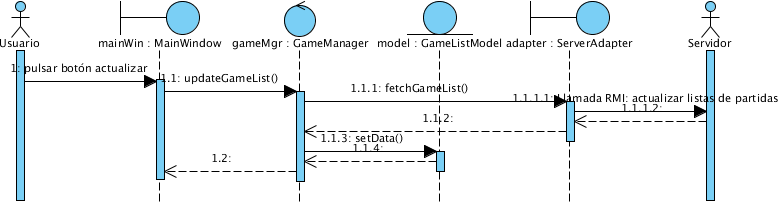
\includegraphics[scale=0.6]{img/ch03devel-listgames.png}
\caption{Diagrama de secuencia de ``Actualizar la lista de partidas''}
\end{figure}

Estando en la ventana principal, el usuario puede realizar una serie de
acciones. Una de ellas puede ser actualizar la lista de partidas mostrada. Ante
esta acción, el gestor de partidas solicitará una nueva lista al servidor a
través del \texttt{ServerAdapter}.

La lista recibida desde el servidor debe ser filtrada y organizada en dos
sublistas: una con partidas abiertas para unirse, y otra con partidas en las
que esté participando el usuario y estén activas en este momento.

Una vez seleccionadas las partidas, éstas son asignadas a dos objetos de tipo
\texttt{GameListModel}. Puesto que las vistas, dos \texttt{JTable}, han sido
configuradas como observadores de estos modelos, su actualización es llevada a
cabo por el \textit{framework} automáticamente.

\subsection{Crear una partida}

\begin{figure}[ht]
\centering
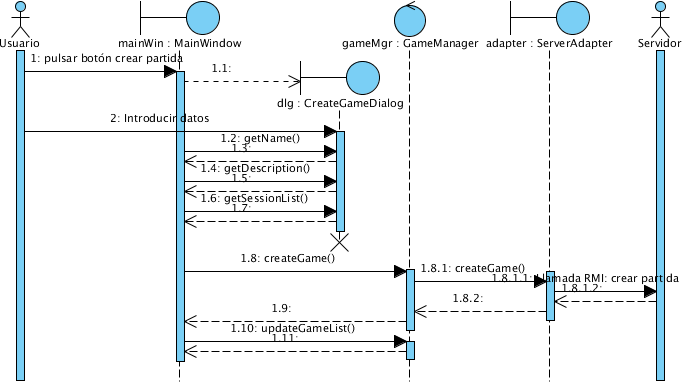
\includegraphics[scale=0.6]{img/ch03devel-creategame.png}
\caption{Diagrama de secuencia de ``Crear una partida''}
\end{figure}

Cuando el usuario seleccione la opción de crear una nueva partida, se le
mostrará una ventana diálogo donde podrá seleccionar los parámetros de esta
nueva partida.

Con estos datos, la ventana principal solicitará al gestor de partidas la
creación de una nueva partida. Si no ocurre ninguna excepción, se realizará una
llamada al caso de uso anterior, actualizar lista de partidas, para que se
actualicen los modelos de datos, y por tanto la interfaz de usuario.

\section{Unirse a una partida}

\begin{figure}[ht]
\centering
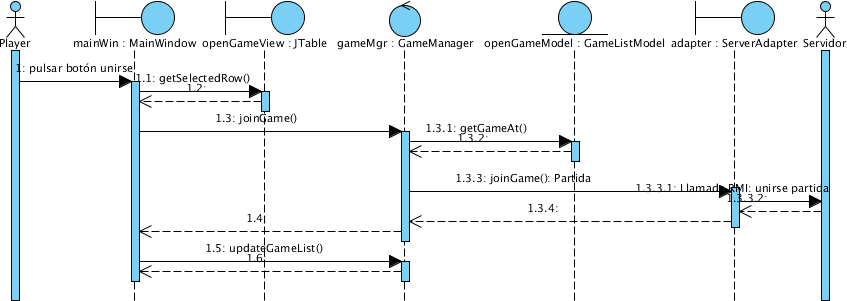
\includegraphics[scale=0.6]{img/ch03devel-joingame.png}
\caption{Diagrama de secuencia de ``Unirse a una partida''}
\end{figure}

Al seleccionar una partida listada en la vista de partidas disponibles, se
activará el botón para unirse a ella. Al pulsar este botón, la ventana
principal obtendrá el índice de la partida seleccionada y llamará a la función
correspondiente del gestor de partidas.

Utilizando el índice proporcionado desde la interfaz, el gestor de partidas
obtendrá el objeto \texttt{GameInfo} que representa a la partida seleccionada.
A continuación pedirá al \texttt{ServerAdapter} que efectúe la unión a la
partida en el servidor.

Al igual que ocurría en el caso de uso anterior, se llamará a la funcionalidad
de actualizar la lista de partidas para que la interfaz muestre los cambios
producidos.

\section{Conectarse a una partida}

\begin{figure}[ht]
\centering
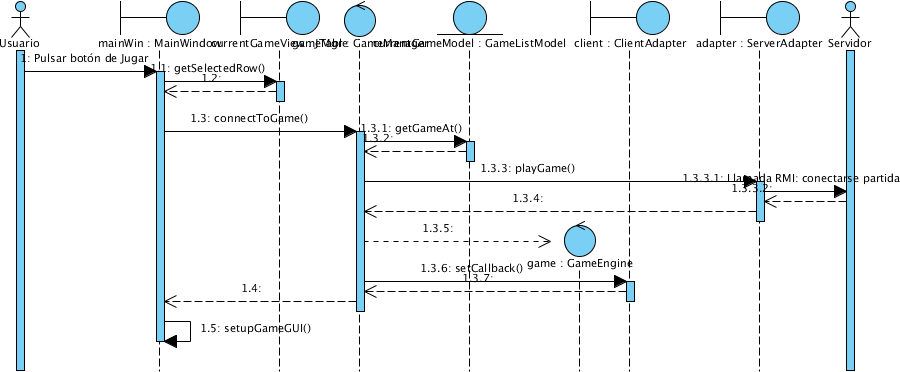
\includegraphics[scale=0.6]{img/ch03devel-playgame.png}
\caption{Diagrama de secuencia de ``Conectarse a una partida''}
\end{figure}

Si se selecciona una partida a la que el usuario ya se haya unido previamente,
podrá entonces ejecutar la acción de jugar en esa partida. Al igual que en el
caso anterior, la ventana principal obtendrá el índice de la partida a partir
de la vista.

El gestor de partidas realizará la petición al servidor de comenzar a jugar en
la partida seleccionada. Es entonces cuando el gestor de partidas creará un
objeto de tipo \texttt{GameEngine} a partir de los datos devueltos por el
servidor.

Esta clase está encargada de toda la lógica del juego, e implementa todos los
casos de uso relacionados con el módulo de juego. Dentro de ella se crean los
dos modelos de datos básicos en cada partida: \texttt{MapModel} y
\texttt{PlayerListModel}.

La clase \texttt{MapModel} almacena la información de los 42 territorios que
tiene una partida. Los datos de cada territorio son accesibles al completo a
través de la función \texttt{getTerritoryAt}. Sin embargo, si se accede a través
de la función \texttt{getValueAt} definida por el \textit{framework}, los datos
devueltos son filtrados de acuerdo a las reglas del juego. Esto es así porque
las vistas usarán esta última función, y de esta forma la vista no necesita
realizar ninguna lógica de control sobre los datos. La clase
\texttt{PlayerListModel} funciona de manera análoga con la lista de jugadores.

El motor del juego también debe responder a las peticiones que llegan del
servidor. Para ello se ha creado la interfaz \texttt{ClientCallback}, la cual
implementa. Una vez creado el objeto de tipo \texttt{GameEngine}, éste es
pasado al \texttt{ClientAdapter} para que redirija las peticiones que lleguen
del servidor.

Finalmente, cuando dominio ha terminado de preparar los datos, la ventana
principal carga la nueva interfaz de partida. Ésta está compuesta por tres
vistas: \texttt{MapView}, \texttt{PlayerView}, y \texttt{TerritoryInfoView}.

Todas estas vistas implementan la interfaz \texttt{TableModelListener}, a la
vez que se registran como observadores de los modelos correspondientes. La
vista \texttt{TerritoryInfoView} muestra información sobre el territorio
seleccionado en el mapa. Por ese motivo, esta clase también debe registrarse
como observador del modelo de selección de la clase \texttt{MapView}.


\chapter{Pruebas de desarrollo}

\section{Clase UserManager}

\subsection{UserManager::registerUser}

{\small
\begin{tabular}{r|l}
Nombre del \textit{tester} & Antonio Gómez Poblete \\
Fecha de asignación & 27 de enero de 2011 \\
Fecha de finalización & 30 de enero de 2011 \\
Código bajo prueba & \texttt{UserManager::registerUser}
\end{tabular}
}

A continuación se detallarán las pruebas de desarrollo (Pruebas unitarias con \textit{Junit}).

Lista de los valores de prueba para cada atributo.
El criterio elegido para todos los valores de prueba (test data) ha sido: Añadir valores interesantes propensos a error (Conjetura de error).

\begin{itemize}
\item \textbf{\texttt{login}}
\subitem \textit{null}
\subitem Cadena vacía
\subitem Usuario existente: \texttt{"JorgeCA"}
\subitem Usuario no existente: \texttt{"LuisAn"}

\item \textbf{\texttt{passwd}}
\subitem \textit{null}
\subitem Cadena vacía
\subitem Cadenas no vacías: \texttt{"jorge"}, \texttt{"luis"}

\item \textbf{\texttt{email}}
\subitem \textit{null}
\subitem Cadena vacía
\subitem Valores incorrectos: \texttt{"jorge"}, \texttt{"jorge@"}, \texttt{"jorge@gmail"}, \texttt{"jorge@gmail."}
\subitem Valores correctos: \texttt{"jorge.colao@gmail.com"}, \texttt{"luis@gmail.com"}
\end{itemize}

La estrategia para obtener los casos de prueba elegida ha sido
\textit{each choice} (Test 1 a 3 y 8 a 12 ) y añadir algunos casos
interesantes (Test 4 a 7).
El test 13 se ha elaborado para ver el comportamiento de registerUser cuando el servidor se ha desconectado.

Para elegir tanto los valores de prueba como los casos de pruebas se ha analizado el comportamiento de este caso de uso (caja blanca). Tras este análisis se ha llegado a la conclusión de que hay en dos lugares en los que se pueden encontrar errores: Si al método registerUser se le da un parámetro erróneo (throw EmptyStringException, MalformedEmailException, NullPointerException), o si el nombre del usuario ya existe en el servidor (throw UserAlreadyExistsException). La primera comprobación es local, por ello si se lanza la excepcion InvalidArgumentException no se hará nada en el servidor y no se analizará si el usuario ya existe o no.

Además, si observamos las comprobaciones que se hacen en el cliente se ve que si login == null, independientemente del valor de los demás atributos se lanzará  NullPointerException, por esa razón es independiente el valor de los demas atributos, lo que hace que muchos casos de prueba no sean necesarios de probar. Por otro lado, para probar qué pasa si el email es \textit{null} el resto de los parámetros deberán ser correctos, lo que añade algunos casos interesantes. Además de con \textit{null} lo comentado en este parrafo sucede con el resto de los parámetros.


Teniendo en cuenta las consideraciones anteriormente mencionadas, la tabla completa de los casos de prueba y los resultados esperados son:

{\footnotesize
\begin{longtable}[c]{lccc}
 & \textbf{Valores de Prueba} & \textbf{Objetivo del test} & \textbf{Resultado esperado} \\
\hline \hline
\endhead

T1 & (vacío, vacío, vacío)  & login & EmptyStringException\\
T2 & (null, null, null) & login & NullPointerException\\
T3 & (JorgeCA, jorge, jorge.colao@gmail.com) & Usuario ya existente & UserAlreadyExistst\\
T4 & (JorgeCA, vacío, jorge.colao@gmail.com) & passwd   & EmptyStringException\\
T5 & (JorgeCA, null, jorge.colao@gmail.com) & passwd   & NullPointerException\\
T6 & (JorgeCA, jorge, vacío) & email   & EmptyStringException\\
T7 & (JorgeCA, jorge, null) & email   & NullPointerException\\
T8 & (JorgeCA, jorge, jorge) & email & MalformedEmailException\\
T9 & (JorgeCA, jorge, jorge@) & email & MalformedEmailException\\
T10 & (JorgeCA, jorge, jorge@gmail) & email & MalformedEmailException\\
T11& (JorgeCA, jorge, jorge@gmail.) & email  & MalformedEmailException\\
T12& (LuisAn, luis, luis@gmail.com) & email  &  El usuario \\
& &  & queda registrado\\
T13& (Angel\&Duran, angel, a@d.com)  & Comportamiento registerUser & RemoteException \\
\hline
\end{longtable}
}

\subsection{UserManager::login}

{\small
\begin{tabular}{r|l}
Nombre del \textit{tester} & Angel Durán Izquierdo \\
Fecha de asignación & 27 de enero de 2011 \\
Fecha de finalización & 2 de febrero de 2011 \\
Código bajo prueba & \texttt{UserManager::createSession}
\end{tabular}
}

A continuación se detallarán las pruebas de desarrollo (Pruebas unitarias con \textit{JUnit}).

Lista de los valores de prueba para cada atributo.
El criterio elegido para todos los valores de prueba (test data) ha sido: Añadir valores interesantes propensos a error (Conjetura de error).

\begin{itemize}
\item \textbf{\texttt{login}}
\subitem \textit{null}
\subitem Cadena vacía
\subitem Usuario existente: \texttt{Angel}
\subitem Usuario no existente: \texttt{ADuran}
\subitem Nombre de usuario registrado pero introducido con mayusculas: \texttt{ADuran}
\subitem Usuario existente con carácteres especiales: \texttt {Angel\&Duran}
\subitem Usuario existente con numeros: \texttt{1111, -1}

\item \textbf{\texttt{passwd}}
\subitem \textit{null}
\subitem Cadena vacía
\subitem Cadenas no vacías: \texttt{angel}
\subitem Cadenas con carácteres especiales: \texttt{22\&22}
\subitem Cadenas con numeros: \texttt{2222}

\end{itemize}

La estrategia para obtener los casos de prueba elegida ha sido
\textit{each choice} eligiendo los casos mas interesantes.

Para elegir tanto los valores de prueba como los casos de pruebas se ha analizado el comportamiento de este caso de uso (caja blanca). Tras este análisis se ha llegado a la conclusión de que hay en dos lugares en los que se pueden encontrar errores: Si al método createSession se le da un parámetro erróneo (throw InvalidArgumentException), o si el nombre del usuario no se ha registrado en el servidor (throw UserAlreadyExistsException).

Por otro lado se comprueba si al crear una sesion cuando ya se existía una, la anterior se cierra correctamente.


Teniendo en cuenta las consideraciones anteriormente mencionadas, la tabla completa de los casos de prueba y los resultados esperados son:

{\footnotesize
\begin{longtable}[c]{lccc}
 & \textbf{Valores de Prueba} & \textbf{Objetivo del test} & \textbf{Resultado esperado} \\
\hline \hline
\endhead

Test1 & (vacío, vacío)  & login-pass & InvalidArgument\\
Test2 & (Aduran, vacío) & pass & InvalidArgument\\
Test3 & (vacío, angel) & login & UserAlreadyExistst\\
Test4 & (Aduran, angel) & login-pass   & Sesión creada correctamente\\
Test5 & (null, angel) & login   & InvalidArgument\\
Test6 & (Aduran, null) & pass   & InvalidArgument\\
Test7 & (null, null) & login-pass   & InvalidArgument\\
Test8 & (ADuran, angel) & login & WrongLoginException\\
Test9 & (Aduran, Angel) & pass & WrongLoginException\\
Test10 & (1111, 22\&22) & login-pass & Sesión creada correctamente\\
Test11& (-1, 2222) & login-pass  & Sesión creada correctamente\\
Test12& (Angel\&Duran, angel) & login  &  Sesión creada correctamente \\
Test13 & (Aduran y ricki, angel y ricki) & Comportamiento createSession & Sesión creada correctamente\\
Test14 & (Aduran, angel) & Comportamiento createSession & RemoteException\\
Test15 & (Aduran, angel) & Comportamiento createSession & Sesión cerrada correctamente\\
Test16 & (Aduran, angel) & Comportamiento createSession & Sesión creada correctamente\\

\hline
\end{longtable}
}

\section{Clase GameManager}

{\small
\begin{tabular}{r|l}
Nombre del \textit{tester} & Jorge Colao Adán \\
& Daniel León Romero\\
Fecha de asignación & 18 de febrero de 2011 \\
Fecha de finalización & 21 de febrero de 2011 \\
Código bajo prueba & \texttt{GameManager}
\end{tabular}
}

En este apartado se hablará sobre las pruebas realizadas con la herramienta \textit{JUnit} sobre esta clase.

La estrategia a seguir para las pruebas de estos apartados será \textit{Each Choice}. La elección de los valores de los parámetos, se realizarán con valores límite para los atributos númericos y valores propensos a error para el resto.

\subsection{GameManager::updateGameList}

En este primer método como no tiene ningún parámetro lo que tenemos que comprobar es que al hacer el test con \textit{JUnit} no salte ninguna excepción. Además, comprobamos que inicialmente el número de partidas a las que se está unido y las partidas disponibles para unirse es igual a cero, y que después de la ejecución de este caso de uso es distinto de cero.

Debido a que con la herramienta \textit{JUnit} no podemos alcanzar una covertura alta, lo que haremos será hacer pruebas exploratorias.

\subsection{GameManager::createGame}

Este método tiene seis parámetros de entrada, por lo que tenemos que utilizar alguna estrategia de generación de casos de prueba. Hemos utilizado \textit{Each Choice} con la herramienta de la página \url{http://161.67.140.42/CombTestWeb/}. Pero comprobando las combinaciones que hemos obtenido nos hemos dado cuenta de que eran poco exahustivas (Test 1 a 3). Debido a este motivo, hemos añadido otros casos de prueba interesantes (Test 4 a 12), como son; probar para que falle cada parámetro independientemente.

Para elegir tanto los valores de prueba como los casos de pruebas de los casos interesantes se ha analizado el comportamiento de este método (mediante caja blanca). Después de analizar el método nos hemos dado cuenta de que pude haber los siguientes errores:
\begin{itemize}
\item NullPointerException
\item EmptyStringException
\item NegativeValueException
\end{itemize}
Esta comprobación es local, por ello si se lanza alguna excepción de las anteriores, no se creará la partida en el servidor.

\begin{itemize}
\item \textbf{\texttt{name}}
\subitem \textit{null}
\subitem Cadena vacía
\subitem Cadena válida: \texttt{"partida"}

\item \textbf{\texttt{description}}
\subitem \textit{null}
\subitem Cadena vacía
\subitem Cadena válida: \texttt{"partida guerra mundo"}

\item \textbf{\texttt{gameSession}}
\subitem \textit{null}
\subitem Fecha: \texttt{"Hora actual"} y \texttt{"01/Marzo/2012 a las 14:00"}

\item \textbf{\texttt{turnTime}}
\subitem Número incorrecto: \texttt{"0"}
\subitem Número correcto. \texttt{"1"} y \texttt{"112"}

\item \textbf{\texttt{defTime}}
\subitem Número incorrecto: \texttt{"0"}
\subitem Número correcto. \texttt{"1"} y \texttt{"20"}

\item \textbf{\texttt{negTime}}
\subitem Número incorrecto: \texttt{"0"}
\subitem Número correcto. \texttt{"1"} y \texttt{"33"}
\end{itemize}

La única comprobación especial que podemos hacer es mirar si salta alguna excepción, si no salta ninguna excepción el método estará correcto, lo que creará una partida en el servidor.

Esta es la tabla de casos de prueba y resultados esperados.

{\footnotesize
\begin{longtable}[c]{lccc}
 & \textbf{Valores de Prueba} & \textbf{Objetivo del test} & \textbf{Resultado esperado} \\
\hline \hline
\endhead

Test1 & ("partida", "partida guerra mundo",  & crear partida & Funcinamiento Correcto \\
 & Fecha\_Posterior, 112, 1, 1) & & \\
Test2 & (null, null, Fecha\_Actual, & name, description & NullPointer\\
 & 1, 20, 33) & & \\
Test3 & (vacío, vacío, & gameSession & NullPointer\\
 & null, 0, 0, 0) & & \\


Test4 & (vacío, vacío,  & name & EmptyString\\
 &  Fecha\_Posterior, 1, 1, 1) & & \\
Test5 & (null, "partida guerra mundo",  & name & NullPointer\\
 &   Fecha\_Posterior, 1, 1, 1) & & \\
Test6 & ("partida", null,  & description  & NullPointer\\
 &  Fecha\_Actual, 1, 1, 33) & & \\
Test7 & ("partida", "partida guerra mundo",  & gameSession & NullPointer\\
 &   null, 1, 1, 33) & & \\
Test8 & ("partida", "partida guerra mundo",  & turnTime & NegativeValue\\
 &   Fecha\_Actual, 0, 20, 33) & & \\
Test9 & ("partida", "partida guerra mundo",  & defTime & NegativeValue\\
 &   Fecha\_Actual, 112, 0, 33) & & \\
Test10 & ("partida", "partida guerra mundo",  & negTime & NegativeValue\\
 &  Fecha\_Actual, 112, 20, 0) & & \\
Test11 & ("partida", "partida guerra mundo",  & crear partida & Funcinamiento Correcto \\
 &  Fecha\_Actual, 112, 20, 33) & & \\
Test12 & ("partida", vacío,   & crear partida & Funcinamiento Correcto \\
 &  Fecha\_Posterior, 1, 1, 1) & & \\

\hline
\end{longtable}
}

\subsection{GameManager::joinGame}

Para este caso de uso tan sólo tenemos un parámetro que es el número del juego al que queremos unirnos. Por este motivo tenemos que comprobar los valores límite de la lista de partidas a unirse. Para representar los valores límite, hemos usado de límite inferior los números ''--1'' y "0", ya que la comparación es que sea menor de "0". Y para el límite superior usaremos el tope de partidas disponibles en el servidor y el tope más uno. En nuestro servidor tenemos dos partidas a las que nos podemos unir, por lo tanto, el tope sería ``1'' y el tope más uno sería ``2''. 

\begin{itemize}
\item \textbf{\texttt{gameSelected}}
\subitem Límite inferior: \texttt{"\--1"} y \texttt{"0"}
\subitem Límite superior: \texttt{"tope = 1"} y \texttt{"tope + 1 = 2"}
\end{itemize}

También tenemos que comprobar que antes de unirnos a la partida tiene que haber al menos una partida a la que podamos unirnos. Y después de unirnos comprobar que el número de filas en la lista de partidas actuales es mayor que antes y la lista de partidas para unirme es menor.
Las posobles excepciones que puede tener este método son:
\begin{itemize}
\item ArrayIndexOutOfBoundsException, para números por debajo del rango.
\item IndexOutOfBoundsException, pra números por encima del rango.
\end{itemize}

Esta es la tabla de casos de prueba y resultados esperados.

{\footnotesize
\begin{longtable}[c]{lccc}
 & \textbf{Valores de Prueba} & \textbf{Objetivo del test} & \textbf{Resultado esperado} \\
\hline \hline
\endhead

Test1 & (-1) & gameIndex (límite inferior) & ArrayIndexOutOfBounds\\
Test2 & (1) & seleccionar segunda partida & Funcionamiento correcto\\
Test3 & (0) & seleccionar primera partida & Funcionamiento correcto\\
Test4 & (2) & gameIndex (límite superior) & IndexOutOfBounds\\

\hline
\end{longtable}
}

\subsection{GameManager::connectToGame}

En este método tenemos dos parámetros, uno es el número de la partida seleccionada para jugar y el otro un evento, que para poder realizar la pruebas tenemos que crearnos una clase privada que implemente \textit{GameEventListener}. De esta forma, nos centramos en el primer parámetro que es el interesante. Como sólo tenemos un parámetro al igual que antes tenemos que sacar los valores límite. En esta ocasión en el servidor tenemos una única partida actual, por lo que el tope es ``0'' y el tope más uno es ``1''.

\begin{itemize}
\item \textbf{\texttt{gameSelected}}
\subitem Límite inferior: \texttt{"\--1"} y \texttt{"0"}
\subitem Límite superior: \texttt{"tope = 0"} y \texttt{"tope + 1 = 1"}
\end{itemize}

Además, antes de conectar tenemos que comprobar que almenos tengamos una partida a la cual podamos conectarnos para jugar y que el objeto GameEngine esté a null y que después de ejecutar el conectar no sea null.

Esta es la tabla de casos de prueba y resultados esperados.

{\footnotesize
\begin{longtable}[c]{lccc}
 & \textbf{Valores de Prueba} & \textbf{Objetivo del test} & \textbf{Resultado esperado} \\
\hline \hline
\endhead

Test1 & (-1, new TestGameEventListener()) & gameIndex (límite inferior) & ArrayIndexOutOfBounds\\
Test2 & (0, new TestGameEventListener()) & seleccionar partida & Funcionamiento correcto\\
Test3 & (1, new TestGameEventListener()) & gameIndex (límite superior) & IndexOutOfBounds\\
Test4 & (0, null) & gameListener & NullPointer\\

\hline
\end{longtable}
}

\subsection{GameManager::disconnectFromGame}

Este método no tiene ningún parámetro de entrada, por lo que para comprobar que funciona correctamente. Tenemos que conectarnos previamante a una partida y luego ejecutar este método, si se lanza la excepción \textit{NullPointerExcepcition}, la ejecución fallará. En caso contrario el método funciona correctamente.



\section{Clase GameListModel}

\subsection{GameListModel::getColumnCount}

{\small
\begin{tabular}{r|l}
Nombre del \textit{tester} & \'Angel Dur\'an Izquierdo\\
Fecha de asignación & 21 de febrero de 2011 \\
Fecha de finalización & 22 de febrero de 2011 \\
Código bajo prueba & \texttt{GameListModel::getColumnCount}
\end{tabular}
}

A continuación se detallarán las pruebas de desarrollo (Pruebas unitarias con \textit{Junit}).

Este m\'etodo no tiene ning\'un parametro por lo que solo se prueba que devuelve el n\'umero correcto de columnas, este dato esta fijado en la clase y no es variable. A su vez se comprueba que no se produce ninguna excepci\'on durante la realizaci\'on de las pruebas.

\subsection{GameListModel::getColumnName}

{\small
\begin{tabular}{r|l}
Nombre del \textit{tester} & \'Angel Dur\'an Izquierdo\\
Fecha de asignación & 21 de febrero de 2011 \\
Fecha de finalización & 22 de febrero de 2011 \\
Código bajo prueba & \texttt{GameListModel::getColumnName}
\end{tabular}
}

A continuación se detallarán las pruebas de desarrollo (Pruebas unitarias con \textit{JUnit}).

Lista de los valores de prueba para cada atributo.
El criterio elegido para todos los valores de prueba (test data) ha sido: Añadir valores interesantes propensos a error (Conjetura de error).

Al m\'etodo se le pasa un entero (col) que indica la columna de la cual queremos recuperar el nombre. 

\begin{itemize}
\item \textbf{\texttt{col}}
\subitem Valor correcto de columna: 0
\subitem Valor negativo: -1
\subitem Valor positivo pero no existe coluna: 6
\end{itemize}

La estrategia para obtener los casos de prueba elegida ha sido
\textit{each choice}.

La tabla completa de los casos de prueba y los resultados esperados son:

{\footnotesize
\begin{longtable}[c]{lccc}
 & \textbf{Valores de Prueba} & \textbf{Objetivo del test} & \textbf{Resultado esperado} \\
\hline \hline
\endhead

Test1 & (0) & col & Devuelve el dato correcto\\
Test2 & (-1) & col & Excepci\'on\\
Test3 & (6) & col & Excepci\'on\\

\hline
\end{longtable}
}

\subsection{GameListModel::getGameAt}

{\small
\begin{tabular}{r|l}
Nombre del \textit{tester} & \'Angel Dur\'an Izquierdo\\
Fecha de asignación & 21 de febrero de 2011 \\
Fecha de finalización & 22 de febrero de 2011 \\
Código bajo prueba & \texttt{GameListModel::getGameAt}
\end{tabular}
}

A continuación se detallarán las pruebas de desarrollo (Pruebas unitarias con \textit{JUnit}).

Lista de los valores de prueba para cada atributo.
El criterio elegido para todos los valores de prueba (test data) ha sido: Añadir valores interesantes propensos a error (Conjetura de error).

Al m\'etodo se le pasa un entero (gameSelected) que indica la posici\'on del juego que se quiere recuperar.

\begin{itemize}
\item \textbf{\texttt{col}}
\subitem Valor correcto de posici\'on del juego: 0
\subitem Valor positivo pero no existe el juego: 20
\end{itemize}

La estrategia para obtener los casos de prueba elegida ha sido
\textit{each choice}.

La tabla completa de los casos de prueba y los resultados esperados son:

{\footnotesize
\begin{longtable}[c]{lccc}
 & \textbf{Valores de Prueba} & \textbf{Objetivo del test} & \textbf{Resultado esperado} \\
\hline \hline
\endhead

Test1 & (0) & gameSelected & Devuelve el juego\\
Test2 & (20) & gameSelected & Excepci\'on\\

\hline
\end{longtable}
}

\subsection{GameListModel::setData}

{\small
\begin{tabular}{r|l}
Nombre del \textit{tester} & \'Angel Dur\'an Izquierdo\\
Fecha de asignación & 21 de febrero de 2011 \\
Fecha de finalización & 22 de febrero de 2011 \\
Código bajo prueba & \texttt{GameListModel::setData}
\end{tabular}
}

A continuación se detallarán las pruebas de desarrollo (Pruebas unitarias con \textit{JUnit}).

Lista de los valores de prueba para cada atributo.
El criterio elegido para todos los valores de prueba (test data) ha sido: Añadir valores interesantes propensos a error (Conjetura de error).

Al m\'etodo se le pasa una lista de juegos (data).

\begin{itemize}
\item \textbf{\texttt{data}}
\subitem Lista correcta de juegos: lista de juegos
\subitem Valor nulo: null
\end{itemize}

La estrategia para obtener los casos de prueba elegida ha sido
\textit{each choice}.

La tabla completa de los casos de prueba y los resultados esperados son:

{\footnotesize
\begin{longtable}[c]{lccc}
 & \textbf{Valores de Prueba} & \textbf{Objetivo del test} & \textbf{Resultado esperado} \\
\hline \hline
\endhead

Test1 & lista de juegos & data & Devuelve el juego\\
Test2 & null & data & InvalidArgument\\

\hline
\end{longtable}
}

\subsection{GameListModel::getRowCount}

{\small
\begin{tabular}{r|l}
Nombre del \textit{tester} & \'Angel Dur\'an Izquierdo\\
Fecha de asignación & 21 de febrero de 2011 \\
Fecha de finalización & 22 de febrero de 2011 \\
Código bajo prueba & \texttt{GameListModel::getRowCount}
\end{tabular}
}

A continuación se detallarán las pruebas de desarrollo (Pruebas unitarias con \textit{JUnit}).

Este m\'etodo devuelve el n\'umero de juegos disponibles, no recibe ning\'un valor por lo que solo se ha realizado la para comprobar que se devuelve el n\'umero correcto de juegos.

\subsection{GameListModel::getValueAt}

{\small
\begin{tabular}{r|l}
Nombre del \textit{tester} & \'Angel Dur\'an Izquierdo\\
Fecha de asignación & 21 de febrero de 2011 \\
Fecha de finalización & 22 de febrero de 2011 \\
Código bajo prueba & \texttt{GameListModel::getValueAt}
\end{tabular}
}

A continuación se detallarán las pruebas de desarrollo (Pruebas unitarias con \textit{JUnit}).

Lista de los valores de prueba para cada atributo.
El criterio elegido para todos los valores de prueba (test data) ha sido: Añadir valores interesantes propensos a error (Conjetura de error).

Al m\'etodo se le pasan dos variables, la primera indica el juego del cual se quiere recuperar la informaci\'on (rowIndex). El segundo parametro indica que tipo de informaci\'on debe devolver el m\'etodo (columnIndex).

\begin{itemize}
\item \textbf{\texttt{rowIndex}}
\subitem Existe la fila: 0,1
\subitem No existe la fila: 10
\end{itemize}

\begin{itemize}
\item \textbf{\texttt{columnIndex}}
\subitem Existe el parametro a devolver: 0,1,2
\subitem No existe el parametro a devolver: 10
\end{itemize}

La estrategia para obtener los casos de prueba elegida ha sido
\textit{pair wise} eligiendo despu\'es los casos interesantes. Los test 5 y 6 son redundantes pero se han elegido
para conseguir una covertura mayor del c\'odigo.

La tabla completa de los casos de prueba y los resultados esperados son:

{\footnotesize
\begin{longtable}[c]{lccc}
 & \textbf{Valores de Prueba} & \textbf{Objetivo del test} & \textbf{Resultado esperado} \\
\hline \hline
\endhead

Test1 & (0,0) & rowIndex y columnIndex & Devuelve el atributo nombre\\
Test2 & (1,10) & columnIndex & No devuelve nada\\
Test3 & (10,1) & rowIndex & Devuelve el juego\\
Test4 & (10,10) & rowIndex y columnIndex & No devuelve nada\\
Test5 & (1,1) & rowIndex y columnIndex & Devuelve el juego\\
Test6 & (0,2) & rowIndex y columnIndex & Devuelve el n\'umero de jugadores\\

\hline
\end{longtable}
}
\section{Clase PlayerListModel}

\subsection{PlayerListModel::PlayerListModel}

{\small
\begin{tabular}{r|l}
Nombre del \textit{tester} & \'Angel Dur\'an Izquierdo\\
Fecha de asignación & 21 de febrero de 2011 \\
Fecha de finalización & 22 de febrero de 2011 \\
Código bajo prueba & \texttt{PlayerListModel::PlayerListModel}
\end{tabular}
}

A continuación se detallarán las pruebas de desarrollo (Pruebas unitarias con \textit{JUnit}).

Lista de los valores de prueba para cada atributo.
El criterio elegido para todos los valores de prueba (test data) ha sido: Añadir valores interesantes propensos a error (Conjetura de error).

Al constructor se le pasa dos parametros, el primero es el player propio (selfPlayer) y el segundo es una lista de usuarios (data).

\begin{itemize}
\item \textbf{\texttt{selfPlayer}}
\subitem Valor correcto: owner
\subitem Valor nulo: null
\end{itemize}

\begin{itemize}
\item \textbf{\texttt{data}}
\subitem Valor correcto: lista de jugadores
\subitem Valor nulo: null
\end{itemize}

La estrategia para obtener los casos de prueba elegida ha sido
\textit{pair wise} seleccionando las combinaciones interesantes.

La tabla completa de los casos de prueba y los resultados esperados son:

{\footnotesize
\begin{longtable}[c]{lccc}
 & \textbf{Valores de Prueba} & \textbf{Objetivo del test} & \textbf{Resultado esperado} \\
\hline \hline
\endhead

Test1 & (owner, lista de jugadores) & selfPlayer y data & El objeto se crea correctamente\\
Test2 & (null, null) & selfPlayer y data & NullPointerException\\

\hline
\end{longtable}
}

\subsection{PlayerListModel::getColumnName}

{\small
\begin{tabular}{r|l}
Nombre del \textit{tester} & \'Angel Dur\'an Izquierdo\\
Fecha de asignación & 21 de febrero de 2011 \\
Fecha de finalización & 22 de febrero de 2011 \\
Código bajo prueba & \texttt{PlayerListModel::getColumnName}
\end{tabular}
}

A continuación se detallarán las pruebas de desarrollo (Pruebas unitarias con \textit{JUnit}).

Lista de los valores de prueba para cada atributo.
El criterio elegido para todos los valores de prueba (test data) ha sido: Añadir valores interesantes propensos a error (Conjetura de error).

Al m\'etodo se le pasa un entero (col) que indica la columna de la cual queremos recuperar el nombre.

\begin{itemize}
\item \textbf{\texttt{col}}
\subitem Valor correcto de columna: 1
\subitem Valor de coluna invalido: 5
\end{itemize}

La estrategia para obtener los casos de prueba elegida ha sido
\textit{each choice}.

La tabla completa de los casos de prueba y los resultados esperados son:

{\footnotesize
\begin{longtable}[c]{lccc}
 & \textbf{Valores de Prueba} & \textbf{Objetivo del test} & \textbf{Resultado esperado} \\
\hline \hline
\endhead

Test1 & (1) & col & Devuelve el dato correcto\\
Test2 & (5) & col & Excepci\'on\\

\hline
\end{longtable}
}

\subsection{PlayerListModel::getPlayerAt}

{\small
\begin{tabular}{r|l}
Nombre del \textit{tester} & \'Angel Dur\'an Izquierdo\\
Fecha de asignación & 21 de febrero de 2011 \\
Fecha de finalización & 22 de febrero de 2011 \\
Código bajo prueba & \texttt{PlayerListModel::getPlayerAt}
\end{tabular}
}

A continuación se detallarán las pruebas de desarrollo (Pruebas unitarias con \textit{JUnit}).

Lista de los valores de prueba para cada atributo.
El criterio elegido para todos los valores de prueba (test data) ha sido: Añadir valores interesantes propensos a error (Conjetura de error).

Al m\'etodo se le pasa un entero (index) que indica la posici\'on del jugador que se quiere recuperar.

\begin{itemize}
\item \textbf{\texttt{index}}
\subitem Valor correcto: 0
\subitem Valor de posici\'on que no existe: 5
\end{itemize}

La estrategia para obtener los casos de prueba elegida ha sido
\textit{each choice}.

La tabla completa de los casos de prueba y los resultados esperados son:

{\footnotesize
\begin{longtable}[c]{lccc}
 & \textbf{Valores de Prueba} & \textbf{Objetivo del test} & \textbf{Resultado esperado} \\
\hline \hline
\endhead

Test1 & (0) & index & Devuelve el jugador correcto\\
Test2 & (5) & index & Excepci\'on\\

\hline
\end{longtable}
}

\subsection{PlayerListModel::setData}

{\small
\begin{tabular}{r|l}
Nombre del \textit{tester} & \'Angel Dur\'an Izquierdo\\
Fecha de asignación & 21 de febrero de 2011 \\
Fecha de finalización & 22 de febrero de 2011 \\
Código bajo prueba & \texttt{PlayerListModel::setData}
\end{tabular}
}

A continuación se detallarán las pruebas de desarrollo (Pruebas unitarias con \textit{JUnit}).

Lista de los valores de prueba para cada atributo.
El criterio elegido para todos los valores de prueba (test data) ha sido: Añadir valores interesantes propensos a error (Conjetura de error).

Al m\'etodo se le pasa una lista de jugadores (data).

\begin{itemize}
\item \textbf{\texttt{data}}
\subitem Lista correcta de jugadores: lista de jugadores
\subitem Valor nulo: null
\end{itemize}

La estrategia para obtener los casos de prueba elegida ha sido
\textit{each choice}.

La tabla completa de los casos de prueba y los resultados esperados son:

{\footnotesize
\begin{longtable}[c]{lccc}
 & \textbf{Valores de Prueba} & \textbf{Objetivo del test} & \textbf{Resultado esperado} \\
\hline \hline
\endhead

Test1 & lista de jugadores & data & setdata correcto\\
Test2 & null & data & Excepci\'on\\

\hline
\end{longtable}
}

\subsection{PlayerListModel::getRowCount}

{\small
\begin{tabular}{r|l}
Nombre del \textit{tester} & \'Angel Dur\'an Izquierdo\\
Fecha de asignación & 21 de febrero de 2011 \\
Fecha de finalización & 22 de febrero de 2011 \\
Código bajo prueba & \texttt{PlayerListModel::getRowCount}
\end{tabular}
}

A continuación se detallarán las pruebas de desarrollo (Pruebas unitarias con \textit{JUnit}).

Este m\'etodo devuelve el n\'umero de jugadores disponibles, no recibe ning\'un valor por lo que solo se ha realizado la para comprobar que se devuelve el n\'umero correcto de jugadores.

\subsection{PlayerListModel::getColumnCount}

{\small
\begin{tabular}{r|l}
Nombre del \textit{tester} & \'Angel Dur\'an Izquierdo\\
Fecha de asignación & 21 de febrero de 2011 \\
Fecha de finalización & 22 de febrero de 2011 \\
Código bajo prueba & \texttt{PlayerListModel::getColumnCount}
\end{tabular}
}

A continuación se detallarán las pruebas de desarrollo (Pruebas unitarias con \textit{Junit}).

Este m\'etodo no tiene ning\'un parametro por lo que solo se prueba que devuelve el n\'umero correcto de columnas, este dato esta fijado en la clase y no es variable. A su vez se comprueba que no se produce ninguna excepci\'on durante la realizaci\'on de las pruebas.

\subsection{PlayerListModel::getValueAt}

{\small
\begin{tabular}{r|l}
Nombre del \textit{tester} & \'Angel Dur\'an Izquierdo\\
Fecha de asignación & 21 de febrero de 2011 \\
Fecha de finalización & 22 de febrero de 2011 \\
Código bajo prueba & \texttt{PlayerListModel::getValueAt}
\end{tabular}
}

A continuación se detallarán las pruebas de desarrollo (Pruebas unitarias con \textit{JUnit}).

Lista de los valores de prueba para cada atributo.
El criterio elegido para todos los valores de prueba (test data) ha sido: Añadir valores interesantes propensos a error (Conjetura de error).

Al m\'etodo se le pasan dos variables, la primera indica el jugador del cual se quiere recuperar la informaci\'on (rowIndex). El segundo parametro indica que tipo de informaci\'on debe devolver el m\'etodo (columnIndex).

\begin{itemize}
\item \textbf{\texttt{rowIndex}}
\subitem Existe la fila: 0
\subitem No existe la fila: 3
\end{itemize}

\begin{itemize}
\item \textbf{\texttt{columnIndex}}
\subitem Existe el parametro a devolver: 0,1,2
\subitem No existe el parametro a devolver: 10
\end{itemize}

La estrategia para obtener los casos de prueba elegida ha sido
\textit{pair wise} eligiendo despu\'es los casos interesantes. Los test 2 y 3 son redundantes pero se han elegido
para conseguir una covertura mayor del c\'odigo.

La tabla completa de los casos de prueba y los resultados esperados son:

{\footnotesize
\begin{longtable}[c]{lccc}
 & \textbf{Valores de Prueba} & \textbf{Objetivo del test} & \textbf{Resultado esperado} \\
\hline \hline
\endhead

Test1 & (0,0) & rowIndex y columnIndex & Devuelve el nombre del jugador\\
Test2 & (0,1) & columnIndex & Devuelve turno del jugador\\
Test3 & (0,2) & rowIndex & Devuelve si el jugador esta conectado\\
Test4 & (3,0) & rowIndex  & IndexOutOfBoundsException\\
Test5 & (0,10) & columnIndex & IndexOutOfBoundsException\\

\hline
\end{longtable}
}

\subsection{PlayerListModel::getActivePlayer}

{\small
\begin{tabular}{r|l}
Nombre del \textit{tester} & \'Angel Dur\'an Izquierdo\\
Fecha de asignación & 21 de febrero de 2011 \\
Fecha de finalización & 22 de febrero de 2011 \\
Código bajo prueba & \texttt{PlayerListModel::getActivePlayer}
\end{tabular}
}

A continuación se detallarán las pruebas de desarrollo (Pruebas unitarias con \textit{Junit}).

Este m\'etodo devuelve el jugador activo en un momento determinando, dicha funci\'on no requiere de parametros por lo que unicamente se prueba que al haber un jugador activo el m\'etodo devuelve este jugador.

\subsection{PlayerListModel::getSelfPlayer}

{\small
\begin{tabular}{r|l}
Nombre del \textit{tester} & \'Angel Dur\'an Izquierdo\\
Fecha de asignación & 21 de febrero de 2011 \\
Fecha de finalización & 22 de febrero de 2011 \\
Código bajo prueba & \texttt{PlayerListModel::getSelfPlayer}
\end{tabular}
}

A continuación se detallarán las pruebas de desarrollo (Pruebas unitarias con \textit{Junit}).

Este m\'etodo devuelve el jugador propio, no recibe ning\'un parametro y por lo tanto se ha probado simplemente que al llamar a la funci\'on devuelve el jugador adecuado.

\subsection{PlayerListModel::getPlayerByName}

{\small
\begin{tabular}{r|l}
Nombre del \textit{tester} & \'Angel Dur\'an Izquierdo\\
Fecha de asignación & 21 de febrero de 2011 \\
Fecha de finalización & 22 de febrero de 2011 \\
Código bajo prueba & \texttt{PlayerListModel::getPlayerByName}
\end{tabular}
}

A continuación se detallarán las pruebas de desarrollo (Pruebas unitarias con \textit{JUnit}).

Lista de los valores de prueba para cada atributo.
El criterio elegido para todos los valores de prueba (test data) ha sido: Añadir valores interesantes propensos a error (Conjetura de error).

Al m\'etodo se le pasa un String (name) que indica el nombre del jugador que se quiere recuperar.

\begin{itemize}
\item \textbf{\texttt{name}}
\subitem Valor correcto : "oponente"
\subitem Valor jugador inexistente: "no existe"
\subitem Valor nulo: null
\end{itemize}

La estrategia para obtener los casos de prueba elegida ha sido
\textit{each choice}.

La tabla completa de los casos de prueba y los resultados esperados son:

{\footnotesize
\begin{longtable}[c]{lccc}
 & \textbf{Valores de Prueba} & \textbf{Objetivo del test} & \textbf{Resultado esperado} \\
\hline \hline
\endhead

Test1 & ("oponente") & name & Devuelve el juego\\
Test2 & ("no existe") & name & No devuelve nada\\
Test2 & (null) & name & Excepci\'on\\

\hline
\end{longtable}
} 
\section{Clase MapModel}

{\small
\begin{tabular}{r|l}
Nombre del \textit{tester} & Antonio Gómez Poblete \\
Fecha de asignación & 21 de febrero de 2011 \\
Fecha de finalización & 25 de febrero de 2011 \\
Código bajo prueba & \texttt{MapModel}
\end{tabular}
}

A diferencia de otras clases como los gestores, la clase \texttt{MapModel} únicamente contiene métodos para implementar el patrón MVC, no  implementa casi ninguna otra funcionalidad. Estos métodos son en su mayoría para acceder a los datos que el modelo proporciona y no filtran los atributos de entrada (en ocasiones no tienen) como pueden hacerlo otras clases de dominio. Por esta razón para comprobar esta clase se va a hacer usa de técnicas de caja blanca , intentando cubrir una máxima cobertura del código.  

A continuación se van a ir mencionando los distintos test que se han realizado a esta clase para obtener un cobertura de un 99 \%, teniendo en cuenta que como precondición debe darse que exista un mapModel (recién creado) y dos jugadores (\texttt{Antonio} y \texttt{Ambrosio}) sin ningún territorio.  


\subsection{MapModelTest::testMapModel} 

En este test se comprueba que el constructor de la clase \texttt{MapModel} funciona adecuadamente. Para ello se pregunta por cada uno de los territorios si  son distintos a \texttt{null} y si tienen el identificador que les corresponde.

\subsection {MapModelTest::testSetData}

En este test se comprueba que si los territorios son asignados nuevamente, la información es correcta.

Este test además de probar la función \texttt{setData}, prueba también el método \texttt{updateTerritory} ya que este es llamado desde \texttt{setData}.

\subsection {MapModelTest::testUpdateTerritory}

En este test se actualiza un territorio existente, para ello se le asigna un jugador (\texttt{Antonio}) y se comprueba que ningún país tienen un jugador salvo el país de \texttt{Antonio}. 

\subsection {MapModelTest::testgetColumnName}

En este test se comprueba que \texttt{testgetColumnName} devuelve el nombre correcto para todos los casos.

\subsection {MapModel::getValueAt}

A diferencia de  los métodos anteriormente mencionados, para probar \texttt{getValueAt} se ha aplicado también un enfoque de caja negra.

El criterio elegido para todos los valores de prueba (test data) ha sido: Añadir valores límite y valores interesantes propensos a error (Conjetura de error)  
\begin{itemize}
\item \textbf{\texttt{rowIndex}}
\subitem  Valores fuera de rango: \texttt{map.getRowCount()}, \texttt{-1}.
\subitem \texttt{0}

\item \textbf{\texttt{columnIndex}}
\subitem  Valores fuera de rango: \texttt{map.getColumnCount()}, \texttt{-1}.
\subitem \texttt{0}
\end{itemize}

La estrategia para obtener los casos de prueba elegida ha sido
\textit{each choice}  y añadir algunos casos interesantes .


Teniendo en cuenta las consideraciones anteriormente mencionadas, la tabla completa de los casos de prueba y los resultados esperados son:

{\footnotesize
\begin{longtable}[c]{lcc}
 & \textbf{Valores de Prueba}  & \textbf{Resultado esperado} \\
\hline \hline
\endhead
Test1 & (-1, 0)  & ArrayIndexOutOfBoundsException\\
Test2 & (\texttt{map.getRowCount()}, 0) &  IndexOutOfBoundsException\\
Test3 & (0, -1)  & IndexOutOfBoundsException\\
Test4 & (0, \texttt{map.getColumnCount()}) &  IndexOutOfBoundsException\\
\hline
\end{longtable}
}

\subsubsection {MapModelTest::testgetValueAt5}

Este test ha sido creado para completar los casos de pruebas antes mencionados y así obtener una mayor cobertura. Además los anteriores test esperaban el mismo resultado (todos producían error). 

En este test los dos jugadores (\texttt{Antonio} y \texttt{Ambrosio}) son asignados a dos territorios. Luego se pregunta por la información de dos territorios (14, 6) y se comprueba que al no tener espías solo se mostrará \texttt{¿?} y el nombre del país.

Para finalizar se añade un espía al jugador \texttt{Antonio} que es el \texttt{selfPlayer} y se comprueba que ahora si es posible saber la información del país (14) también se comprueba que  todos los atributos de este son correctos.






\section{Clase TerritoryDecorator}

{\small
\begin{tabular}{r|l}
Nombre del \textit{tester} & Antonio Gómez Poblete \\
Fecha de asignación & 21 de febrero de 2011 \\
Fecha de finalización & 25 de febrero de 2011 \\
Código bajo prueba & \texttt{TerritoryDecorator}
\end{tabular}
}

Gran parte de la lógica  de \texttt{TerritoryDecorator} ha sido ya probada al realizar los casos de pruebas descritos en la sección anterior, 90\% de cobertura.
No obstante quedan algunas funcionalidades sin probar que se describirán a continuación con los siguientes test (se llegará a un 99\%). 

Para realizar todos los test partimos como precondición (método \texttt{setUp()})que se ha creado un \texttt{MapModel}, que existe el jugador \texttt{selfPlayer} y que a dos territorios se les ha asignado jugador.  

\subsection{TerritoryDecoratorTest::testgetclone1}

En este test se clonan tres territorios (0, 6, 14) y se comprueba que el identificador del original y la copia sean el mismo. También se comprueba que los territorios copiados sean los mismo que los originales llamando directamente a la función \texttt{equal}, de  este modo en este  test se comprobará  el \texttt{clone} y el \texttt{equal} de la clase \texttt{TerritoryDecorator}.


\subsection{TerritoryDecoratorTest::testgetEqual1}

En este test se comparan  territorios diferentes (6, 0, 14) con la función \texttt{equal}. Así se comprobarán que ambas posibilidades (true, false) del \texttt{equal} funcionan correctamente.
 
\subsection{TerritoryDecoratorTest::testgetName1} 

El objetivo aquí es comprobar que funciona bien el \texttt{getName} de territorio. Para ello se comprueba que el nombre de dos países es diferente (14, 6).

\subsection{TerritoryDecoratorTest::testgetAdjacentTerritories1}

En este test se comprueba que la función \texttt{getAdjacentTerritories} se comporta correctamente, para ello realizamos algunos test intentando probar las dos posibilidades (ser o no adyacente a un país). 

\begin{itemize} 

\item Se comprueba que \texttt{getAdjacentTerritories()} no devuelva \texttt{null}.

\item Se comprueba que el territorio 0 es adyacente al 1 y el 1 al 0.
	
\item Se comprueba que el territorio 0 no es adyacente al 30.
	
\item Se comprueba que el territorio 6  es adyacente al 0 y el 0 al 6.
	
\item Se comprueba que el territorio 6 no es adyacente al 17.	

\end{itemize}

\section{Clase GameEngine}

{\small
\begin{tabular}{r|l}
Nombre del \textit{tester} & Jorge Colao Adán \\
& Daniel León Romero\\
Fecha de asignación & 1 de marzo de 2011 \\
Fecha de finalización & 7 de marzo de 2011 \\
Código bajo prueba & \texttt{GameEngine}
\end{tabular}
}

En este apartado se hablará sobre las pruebas realizadas con la herramienta \textit{JUnit} sobre esta clase.

La estrategia a seguir para las pruebas de estos apartados será \textit{Each Choice}. La elección de los valores de los parámetos, se realizarán con valores límite para los atributos númericos y valores propensos a error para el resto.

A la hora de realizar las pruebas en la clase GameEngine tenemos unos atributos privados a los que no podemos acceder. Para acceder a ellos se necesita la clase \textit{PrivateAccesor.java}, disponible en la página \url{http://onjava.com/pub/a/onjava/2003/11/12/reflection.html?page=2}. Por ejemplo, para acceder a la variable mCurrentAttack de la clase GameEngine, se tendría declarar un objeto de esta manera:
\begin{verbatim}
Object o = PrivateAccessor.getPrivateField(gameEngine, 
	"mCurrentAttack");
\end{verbatim}

Para poder probar los ataques primero tenemos que conectarnos a la partida. La conexión se realiza con el método connectToGame que tiene como argumentos el número de la partida a la que hay que conectarse y un objeto de la clase \textit{GameEventListener}. Para crear este objeto tenemos que crear una clase privada que implemente \textit{GameEventListener}.

\subsection{GameEngine::attackTerritory}

Este método tiene seis parámetros de entrada, por lo que tenemos que utilizar alguna estrategia de generación de casos de prueba. Hemos utilizado \textit{Each Choice}, combinando las entradas para que falle una y sólo una, en cada caso de prueba y poder saber en donde esta el error.

Para elegir tanto los valores de prueba como los casos de pruebas de los casos interesantes se ha analizado el comportamiento de este método (mediante caja blanca). Después de analizar el método nos hemos dado cuenta de que pude haber los siguientes errores:
\begin{itemize}
\item PendingAttackException
\item ArrayIndexOutOfBoundsException
\item IndexOutOfBoundsException
\item UnocupiedTerritoryException
\item NegativeValueException
\item NotEnoughUnitsException
\item InvalidTerritoryException
\end{itemize}
Esta comprobación es local, por ello si se lanza alguna excepción de las anteriores, no se realizará el ataque.

Estos son los valores de los atributos para los casos de prueba:
\begin{itemize}
\item \textbf{\texttt{src}}
\subitem Número incorrecto: \texttt{"\--1"}, \texttt{"41"} y \texttt{"42"}
\subitem Número correcto: \texttt{"0"}, territorio en el que se encuetra \textit{JorgeCA}

\item \textbf{\texttt{dst}}
\subitem Número incorrecto: \texttt{"\--1"}, \texttt{"0"}, \texttt{"41"} y \texttt{"42"}
\subitem Número correcto: \texttt{"2"}, territorio en el que se encuetra \textit{Aduran}

\item \textbf{\texttt{soldiers}}
\subitem Número incorrecto: \texttt{"\--1"} y \texttt{"21"}
\subitem Número correcto: \texttt{"0"} y \texttt{"20"}

\item \textbf{\texttt{cannons}}
\subitem Número incorrecto: \texttt{"\--1"} y \texttt{"7"}
\subitem Número correcto: \texttt{"0"} y \texttt{"6"}

\item \textbf{\texttt{missiles}}
\subitem Número incorrecto: \texttt{"\--1"} y \texttt{"2"}
\subitem Número correcto: \texttt{"0"} y \texttt{"1"}

\item \textbf{\texttt{icbm}}
\subitem Número incorrecto: \texttt{"\--1"} y \texttt{"7"}
\subitem Número correcto: \texttt{"0"} y \texttt{"6"}
\end{itemize}

La tabla siguiente recoge los resultados esperados.

{\footnotesize
\begin{longtable}[c]{lccc}
 & \textbf{Valores de Prueba} & \textbf{Objetivo del test} & \textbf{Resultado esperado} \\
\hline \hline
\endhead

Test1 & (0, 2, 0, 0, 1, 6)  & realizar ataque & Funcinamiento Correcto\\
Test2 & (0, 2, 0, 0, 1, 6)  & realizar 2 ataques & PendingAttack\\
Test3 & (-1, 2, 0, 0, 1, 6)  & src & ArrayIndexOutOfBounds\\
Test4 & (42, 2, 0, 0, 1, 6)  & src & IndexOutOfBounds\\
Test5 & (41, 2, 0, 0, 1, 6)  & src & UnocupiedTerritory\\
Test6 & (0, -1, 0, 0, 1, 6)  & dst  & ArrayIndexOutOfBounds\\
Test7 & (0, 42, 0, 0, 1, 6)  & dst & IndexOutOfBounds\\
Test8 & (0, 0, 0, 0, 1, 6)  & dst & InvalidTerritory\\
Test9 & (0, 2, -1, 0, 1, 6)  & soldiers & NegativeValue\\
Test10 & (0, 2, 21, 0, 1, 6)  & negTime & NotEnoughUnits\\
Test11 & (0, 2, 20, -1, 1, 6)  & cannons & NegativeValue\\
Test12 & (0, 2, 20, 7, 1, 6)  & cannons & NotEnoughUnits\\
Test13 & (0, 2, 20, 6, -1, 6)  & missiles & NegativeValue\\
Test14 & (0, 2, 20, 6, 2, 6)  & missiles & NotEnoughUnits\\
Test15 & (0, 2, 20, 6, 1, -1)  & icbm & NegativeValue\\
Test16 & (0, 2, 20, 6, 1, 7)  & icbm & NotEnoughUnits\\
Test17 & (0, 2, 0, 0, 0, 0)  & realizar ataque & Funcinamiento Correcto\\
Test18 & (0, 2, 20, 6, 0, 0)  & realizar ataque & Funcinamiento Correcto\\

\hline
\end{longtable}
}


\subsection{GameEngine::territoryUnderAttack}

Este método tiene tres parámetros de entrada, por lo que se utilizará \textit{Each Choice}. Combinando las entradas para que falle una y sólo una, en cada caso de prueba y poder saber en donde está el error.

Para elegir tanto los valores de prueba como los casos de pruebas de los casos interesantes se ha analizado el comportamiento de este método (mediante caja blanca). Después de analizar el método nos hemos dado cuenta de que sólo pude darse la excepción de \textit{NullPointerException}.

Esta comprobación es local, por ello si se lanza la excepción anterior, no se informará de que te quieren atacar.

Estos son los valores de los atributos para los casos de prueba:
\begin{itemize}
\item \textbf{\texttt{src}}
\subitem Territorio 2 de Aduran
\subitem null

\item \textbf{\texttt{dst}}
\subitem Territorio 0 de JorgeCA
\subitem null

\item \textbf{\texttt{arsenal}}
\subitem Arsenal(5, 4, 1, 0)
\subitem null
\end{itemize}

La tabla siguiente recoge los resultados esperados, para los casos de prueba.

{\footnotesize
\begin{longtable}[c]{lccc}
 & \textbf{Valores de Prueba} & \textbf{Objetivo del test} & \textbf{Resultado esperado} \\
\hline \hline
\endhead

Test1 & (T2\_Aduran, T0\_JorgeCA, Arsenal) & informar del ataque & Funcinamiento Correcto\\
Test2 & (null, T0\_JorgeCA, Arsenal) & src & NullPointer\\
Test3 & (T2\_Aduran, null, Arsenal) & dst & NullPointer\\
Test4 & (T2\_Aduran, T0\_JorgeCA, null) & arsenal & NullPointer\\

\hline
\end{longtable}
}

\subsection{GameEngine::acceptAttack}

Este método es una respuesta a al método anterior. No tiene ningún parámetro de entrada, por lo que para poder probarlo sólo podemos comprobar que antes de realizar este método la variable \textit{mCurrentAttack} no sea null y después de ejecutarlo que sea null.

Analizando el comportamiento del método se puede observar que solamente puede dar un error, \textit{OutOfTurnException}.

Esta comprobación es local, por ello si se lanza la excepción OutOfTurnException, no se aceptará el ataque.

Se han realizado dos casos de prueba:
\begin{itemize}
\item Ejecutando primero el método territoryUnderAttack. El cuál da un valor la variable mCurrentAttack y el método aceptar ataque no da error.
\item Sin ejecutar primero el método territoryUnderAttack. En este caso no se le da valor a la varible mCurrentAttack y como es null falla la ejecución de aceptar ataque.
\end{itemize}

\subsection{GameEngine::requestNegotiation}

Al igual que el método anterior, también es la respuesta al método \textit{territoryUnderAttack}. Como valores de entrada tiene dos parámetos:
\begin{itemize}
\item \textbf{\texttt{money}}
\subitem Número incorrecto: \texttt{"\--1"} y \texttt{"201"}
\subitem Número correcto: \texttt{"0"} y \texttt{"200"}

\item \textbf{\texttt{sodiers}}
\subitem Número incorrecto: \texttt{"\--1"} y \texttt{"21"}
\subitem Número correcto: \texttt{"0"} y \texttt{"20"}
\end{itemize}

Los posibles excepciones que pueden lanzarse al ejecutar este método son:
\begin{itemize}
\item OutOfTurnException
\item NegativeValueException
\item NotEnoughUnitsException
\item NotEnoughMoneyException
\item NullPointerException
\end{itemize}

\newpage
La tabla siguiente recoge los resultados esperados.

{\footnotesize
\begin{longtable}[c]{lccc}
 & \textbf{Valores de Prueba} & \textbf{Objetivo del test} & \textbf{Resultado esperado} \\
\hline \hline
\endhead

Test1 & (0, 20) & pedir negociación & Funcinamiento Correcto\\
Test2 & (0, 20) & (*) & NullPointer\\
Test3 & (-1, 0) & money & NegativeValue\\
Test4 & (201, 0) & money & NotEnoughMoney\\
Test5 & (200, -1) & soldiers & NegativeValue\\
Test6 & (200, 21) & soldiers & NotEnoughUnits\\

\hline
\end{longtable}
}

(*)El caso de prueba; Test2 es igual que el primero, pero no se ha realizado el \textit{territoryUnderAttack}, por lo que la variable \textit{mCurrentAttack} es null.

\subsection{GameEngine::resolveAttack}
\subsection{GameEngine::resolveNegotiation}



\chapter{Pruebas exploratorias}

\section{Registrarse}

A continuación se muestra un guión de pruebas exploratorias para cada uno de los escenarios posibles:
\begin{enumerate}
\item Todos los datos son válidos y el usuario no existe.
	\begin{itemize}
	\item Acciones previas: El servidor debe estar funcionando y no tener un usuario con el nombre LuisAn.
	\item Acciones de prueba : En la ventana de inicio pinchamos en registrarnos y rellenamos el diálogo que nos aparecerá con los siguientes valores: LuisAn, luis, luis@gmail.com.
	\item Resultados esperados : Tras pulsar en aceptar  desaparecerá el diálogo de registro y en la parte superior de la ventana de inicio nos aparecerá en verde \emph {Usuario registrado con éxito} y en el campo Login, el nombre del nuevo usuario .
	\end{itemize}

\item Todos los datos son válidos, pero el usuario existe.
	\begin{itemize}
	\item Acciones previas: El servidor debe estar funcionando y  tener un usuario con el nombre JorgeCA.
	\item Acciones de prueba : En la ventana de inicio pinchamos en registrarnos y rellenamos el diálogo que nos aparecerá con los siguientes valores: JorgeCA, jorge, jorge.colao@gmail.com.
	\item Resultados esperados : Tras pulsar en aceptar desaparecerá el diálogo de registro y en la parte superior de la ventana de inicio nos aparecerá en rojo \emph {El usuario seleccionado ya éxite}.
	\end{itemize}

\item Algún dato introducido en el diálogo no ha sido introducido, independientemente de que el usuario exista o no.
	\begin{itemize}
	\item Acciones previas: El servidor debe estar funcionando.
	\item Acciones de prueba : En la ventana de inicio pinchamos en registrarnos y rellenamos el diálogo que nos aparecerá con los siguientes valores: JorgeCA, jorge@gmail.com, cadena vacía.
	\item Resultados esperados : Tras pulsar en aceptar desaparecerá el diálogo de registro y aparecerá un panel de error mostrando \emph{Debes de rellenar todos los parámetros}. Después de pulsar aceptar en el panel, volverá a aparecer el diálogo. Esto sucederá hasta que los datos sean correctos o demos a cancelar.
	\end{itemize}

\item Dirección de email mal escrita, independientemente de que el usuario exista o no.
	\begin{itemize}
	\item Acciones previas: El servidor debe estar funcionando.
	\item Acciones de prueba : En la ventana de inicio pinchamos en registrarnos y rellenamos el diálogo que nos aparecerá con los siguientes valores: JorgeCA, jorge@gmail., jorge.
	\item Resultados esperados : Tras pulsar en aceptar desaparecerá el diálogo de registro y aparecerá un panel de error mostrando \emph{Dirección de email mal escrita}. Después de pulsar aceptar en el panel, volverá a aparecer el diálogo. Esto sucederá hasta que los datos sean correctos o demos a cancelar.
	\end{itemize}
\end{enumerate}

 \subsubsection{Iniciar sesión}

A continuación se muestra un guión de pruebas exploratorias para cada uno de los escenarios posibles:
\begin{enumerate}
\item El usuario esta registrado en el servidor
	\begin{itemize}
	\item Acciones previas: El servidor debe estar funcionando y el usuario debe estar registrado en el mismo.
	\item Acciones de prueba : En la ventana de inicio introducimos en el campo de Login la cadena Aduran y en el campo de Contraseña la cadena angel.
	\item Resultados esperados : Tras pulsar en aceptar la ventana de login desaparecerá y se abrirá la ventana de juego.
	\end{itemize}
\item El usuario no esta registrado en el servidor.
	\begin{itemize}
	\item Acciones previas: El servidor debe estar funcionando y no tener un usuario con el nombre ADuran.
	\item Acciones de prueba : En la ventana de login introducimos el usuario ADuran y la Contraseña angel.
	\item Resultados esperados : Tras pulsar en Aceptar aparece un mensaje de error en la parte superior de la ventana, este mensaje es: \emph {Contraseña o login Erroneos}.
	\end{itemize}

\item Falta algun dato por introducir.
	\begin{itemize}
	\item Acciones previas: El servidor debe estar funcionando.
	\item Acciones de prueba : En la ventana de login introducimos el nombre de usuario Aduran en el campo Login y dejamos el campo Contraseña vacío.
	\item Resultados esperados : Tras pulsar en Aceptar aparece un mensaje de error en la parte superior de la ventana, este mensaje es: \emph {Contraseña o login Erroneos}.
	\end{itemize}
\end{enumerate}


\section{Actualizar la lista de partida}

Una vez logeado el usuario correctamente la fución actualizar la lista de partidas, se ejecuta automáticamente.

Guión de pruebas exploratorias para el método actualizar lista de partidas:

\begin{enumerate}
\item Pulsamos el botón ''Actualizar lista'', estando en hora para jugar una partida.
	\begin{itemize}
	\item Acciones previas: El servidor debe estar funcionando y habernos logeado con éxito.
	\item Acciones de prueba: Pulsamos el botón de ''Actualizar lista''.
	\item Resultados esperados: Tras pulsar el botón, aparecerán las dos litas de partidas, tanto las actuales (si estamos en hora) como las disponible para unirse (si no se han pasado la horas de juego y tiene territorios libres).
	\end{itemize}
\item Pulsamos el botón ''Actualizar lista'', no estando en hora para jugar una partida
	\begin{itemize}
	\item Acciones previas: El servidor debe estar funcionando y habernos logeado con éxito.
	\item Acciones de prueba: Pulsamos el botón de ''Actualizar lista''.
	\item Resultados esperados: Tras pulsar el botón, aparecen las partidas libres pero no las partidas actuales, ya que ho hay ninguna en hora.
	\end{itemize}
\end{enumerate}

\section{Crear una partida}

Guión de pruebas exploratorias para el método crear una partida:

\begin{enumerate}
\item Error la crear una partida con campos vacíos.
	\begin{itemize}
	\item Acciones previas: El servidor debe estar funcionando, haberse logeado con éxito y haber pulsado el botón ''Crear partida'' de la barra de herramientas.
	\item Acciones de prueba: En el dialogo de nueva partida se pulsa directamente en ''Crear Partida'', dejando en blanco los campos nombre, descripción y fecha, porque los demás estan por defecto a 60 segundos.
	\item Resultados esperados: No se crea la nueva partida y muesta el mensaje de error: ''¡Datos erróneos o insuficientes!''.
	\end{itemize}
	
\item Crear una partida, con descripción vacía.
	\begin{itemize}
	\item Acciones previas: El servidor debe estar funcionando, haberse logeado con éxito y haber pulsado el botón ''Crear partida'' de la barra de herramientas.
	\item Acciones de prueba: En el dialogo de nueva partida se escribe el nombre ''partida'' para el campo nombre de la partida y se añade la fecha actual. Los tiempos de juego se quedarán por defecto a 60 segundos. Se pulsa en ''Crear Partida'', dejando en blanco el campo descripción.
	\item Resultados esperados: Se crea una nueva partida, llamada "partida". En nuestro servidor de prueba no esta implementado la creación de una nueva partida, pero con el servidor del grupo de \textit{Jorge Barco} si funciona.
	\end{itemize}
	
\item Crear una partida, rellenando todos los campos.
	\begin{itemize}
	\item Acciones previas: El servidor debe estar funcionando, haberse logeado con éxito y haber pulsado el botón ''Crear partida'' de la barra de herramientas.
	\item Acciones de prueba: En el dialogo de nueva partida se escribe el nombre ''partida'' para el campo nombre de la partida, como descripción se ha puesto ''partida guera mundo'' y se añade la fecha actual. Los tiempos de juego se quedarán por defecto a 60 segundos. Se pulsa en ''Crear Partida''.
	\item Resultados esperados: Se crea una nueva partida, llamada "partida" y con la descripción ''partida guera mundo''.
	\end{itemize}
\end{enumerate}

El problema de las excepciones de rango de los camos de tiempo, no se puede producir, porque en la interzar se evita que se puedan poner números menores de 1.

\subsection{Feedback}

Al realizar la pruebas exploratorias de este método nos dimos cuenta que se podian crear partidas con campos indispensables vacíos. Por lo que se informó al desarrollador pertinente.

\section{Unirse a una partida}

Guión de pruebas exploratorias para el método unirse a una partida:

\begin{enumerate}
\item Pulsamos el botón ''Unirse a la partida'', habiendo seleccionado una partida.
	\begin{itemize}
	\item Acciones previas: El servidor debe estar funcionando, habernos logeado con éxito y haber una partida libre disponible.
	\item Acciones de prueba: Seleccionamos una partida a la que queremos unirnos y luego pulsamos el botón de ''Unirse a la partida''.
	\item Resultados esperados: Si la partida a la que nos vamos a unir está en hora, nos saldra un mensaje para si queremos jugar. En cambio si no está en hora actualizará las dos listas.
	\end{itemize}
\item Pulsamos el botón ''Unirse a la partida'', sin haber seleccionado una partida.
	\begin{itemize}
	\item Acciones previas: El servidor debe estar funcionando, habernos logeado con éxito y haber una partida libre disponible.
	\item Acciones de prueba: Pulsamos el botón de ''Unirse a la partida'' (aunque no está visible).
	\item Resultados esperados: La interfaz muestra un diálogo en el que indica que falta seleccionar una partida.
	\end{itemize}
\end{enumerate}

En realidad el fallo comprobado en la parte de Pruebas de desarrollo, no se puede dar porque la interfaz no lo permite.

\section{Conectarse a una partida}

Guión de pruebas exploratorias para el método conectarse a una partida:

\begin{enumerate}
\item Pulsamos el botón ''Conectarse a partida'', habiendo seleccionado una partida.
	\begin{itemize}
	\item Acciones previas: El servidor debe estar funcionando, habernos logeado con éxito y haber una partida disponible.
	\item Acciones de prueba: Seleccionamos la partida a la que queremos conectarnos para jugar y luego pulsamos el botón de ''Conectarse a partida''.
	\item Resultados esperados: Se cambia la interfaz mostrando la ventana de juego.
	\end{itemize}
\item Pulsamos el botón ''Conectarse a partida'', sin haber seleccionado una partida.
	\begin{itemize}
	\item Acciones previas: El servidor debe estar funcionando, habernos logeado con éxito y haber una partida disponible.
	\item Acciones de prueba: Pulsamos el botón de ''Conectarse a partida'' (aunque aparece desactivado).
	\item Resultados esperados: La interfaz muestra un diálogo en el que indica que falta seleccionar una partida.
	\end{itemize}
\end{enumerate}

En realidad el fallo comprobado en la parte de Pruebas de desarrollo, no se puede dar porque la interfaz no lo permite.

\section{Atacar un territorio}

Guión de pruebas exploratorias para el método atacar un territorio:

\begin{enumerate}
\item Atacar desde un territorio propio.
	\begin{itemize}
	\item Acciones previas: El servidor debe estar funcionando, haberse logeado con éxito y haberse conectado una partida.
	\item Acciones de prueba: Una vez que se está en la partida, se selecciona el territorio (uno propio, ''Gran Bretaña de JorgeCA'') desde el que quieres atacar y se pulsa el botón ''Atacar''. Se muestra el diálogo de atacar, en el que se elige el territorio destino del ataque (''Europa del Norte''). Las tropas con las que se ataca: 6 soldados y 2 cañones. Por último se pulsa el botón ''Aceptar''.
	\item Resultados esperados: No se muestra ningún diálogo de error.
	\end{itemize}
\item Atacar desde un territorio vacío.
	\begin{itemize}
	\item Acciones previas: El servidor debe estar funcionando, haberse logeado con éxito y haberse conectado una partida.
	\item Acciones de prueba: Una vez que se está en la partida, se selecciona un territorio vacío (''Europa Occidental'') desde el que quieres atacar y se pulsa el botón ''Atacar''. 
	\item Resultados esperados: No se realiza ninguna acción, puesto que el territorio no es del usuario.
	\end{itemize}
\item Atacar desde un territorio de un contrincante.
	\begin{itemize}
	\item Acciones previas: El servidor debe estar funcionando, haberse logeado con éxito y haberse conectado una partida.
	\item Acciones de prueba: Una vez que se está en la partida, se selecciona un territorio de un contrincante (''Europa del Norte'') desde el que quieres atacar y se pulsa el botón ''Atacar''. 
	\item Resultados esperados: No se realiza ninguna acción, puesto que el territorio no es del usuario.
	\end{itemize}
\end{enumerate}

Los fallos comprobados en las pruebas de desarrollo con \textit{JUnit} no se darán ya que el número mínimo de las tropas del arsenal es cero y el máximo, el disponible para ese territorio.

\section{Comprar refuerzos}

Guión de pruebas exploratorias para el método Comprar refuerzos. Entre paréntesis se muestran los valores de ciertos parámetros utilizados con el servidor de prueba (en partidas
reales estos parámetros son variables):


\begin{enumerate}
\item Pulsamos el botón ''Comprar refuerzos'', habiendo seleccionado un país que nos pertenece.
	\begin{itemize}
	\item Acciones previas: El servidor debe estar funcionando, habernos logeado con éxito (como usuario JorgeCA) y conectado a una partida (game01).
	\item Acciones de prueba: Una vez en la  partida, seleccionamos un país que nos pertenece (Gran Bretaña) y pulsamos el botón ``Comprar refuerzos''.
Aparecerá el diálogo comprar refuerzos. En él introducimos que deseamos comprar 2 soldados y pulsamos ``Aceptar''
	\item Resultados esperados: Se cambia la interfaz mostrando la ventana de juego y los datos de dinero y tropas actualizados.
	\end{itemize}
\item No es posible pulsar el botón ``Comprar refuerzos'' en ninguna otra situación, puesto que la interfaz no lo permite.
\item Tampoco es posible la introducción de parámetros erróneos a la hora de elegir las tropas, también debido a la interfaz.

\end{enumerate}


\section{Mover tropas}

Guión de pruebas exploratorias para el método moveUnits. Entre paréntesis se muestran los valores de ciertos parámetros utilizados con el servidor de prueba (en partidas
reales estos parámetros son variables):


\begin{enumerate}
\item Pulsamos el botón ''Mover tropas'', habiendo seleccionado un país que nos pertenece.
	\begin{itemize}
	\item Acciones previas: El servidor debe estar funcionando, habernos logeado con éxito (como usuario JorgeCA) y conectado a una partida (game01).
	\item Acciones de prueba: Una vez en la  partida, seleccionamos un país que nos pertenece (Gran Bretaña) y pulsamos el botón ``Mover tropas''.
Aparecerá el diálogo mover tropas. En él seleccionamos como destino ``Iceland'' , seleccionamos las tropas a mover (4 soldados, un cañón de 1 uso, tres de 3 usos y 2 ICBMs, 
por ejemplo) y pulsamos ``Aceptar''
	\item Resultados esperados: Se cambia la interfaz mostrando la ventana de juego y los datos de tropas actualizados.
	\end{itemize}
\item No es posible pulsar el botón ``Mover unidades'' en ninguna otra situación, puesto que la interfaz no lo permite.
\item Tampoco es posible la introducción de parámetros erróneos a la hora de elegir las tropas o el territorio destino, también debido a la interfaz.

\end{enumerate}


\section{Enviar espía}

Guión de pruebas exploratorias para el método deploySpy. Entre paréntesis se muestran los valores de ciertos parámetros utilizados con el servidor de prueba (en partidas
reales estos parámetros son variables):

\begin{enumerate}
\item Pulsamos el botón ''Enviar espía'', habiendo seleccionado un país que no nos pertenece y teniendo dinero suficiente para comprar un espía.
	\begin{itemize}
	\item Acciones previas: El servidor debe estar funcionando, habernos logeado con éxito (como usuario JorgeCA) y conectado a una partida (game01).
	\item Acciones de prueba: Una vez en la  partida, seleccionamos un país que no nos pertenece (España) y pulsamos el botón ``Enviar espía''.     
	\item Resultados esperados: El espía es enviado y se mostrará la pantalla de juego con los gallifantes actualizados
	\end{itemize}
\item Pulsamos el botón ''Enviar espía'', habiendo seleccionado un país que no nos pertenece sin tener dinero suficiente.
	\begin{itemize}
	\item Acciones previas: El servidor debe estar funcionando, habernos logeado con éxito (como usuario JorgeCA) y haber una partida disponible.
	\item Acciones de prueba: Una vez en la  partida, seleccionamos un país que no nos pertenece (España) y pulsamos el botón ``Enviar espía''.     
	\item Resultados esperados: Aparecerá un diálogo informándonos de que no tenemos dinero suficiente para llevar a cabo la acción.
	\end{itemize}
\item No es posible pulsar el botón ``Enviar espía'' en ninguna otra situación, puesto que la interfaz no lo permite.

\end{enumerate}


\section{Comprar Territorio}

Guión de pruebas exploratorias para el método buyTerritory. Entre paréntesis se muestran los valores de ciertos parámetros utilizados con el servidor de prueba (en partidas
reales estos parámetros son variables):

\begin{enumerate}
\item Pulsamos el botón ``Comprar territorio'', habiendo seleccionado un país que no tiene dueño y es adyacente a uno nuestro.
	\begin{itemize}
	\item Acciones previas: El servidor debe estar funcionando, habernos logeado con éxito (como usuario JorgeCA)  y conectado a una partida.
	\item Acciones de prueba: Una vez en la  partida, seleccionamos un país que no nos pertenece (España). Pulsamos el botón ``Comprar Territorio''. 
	\item Resultados esperados: Se cambia la interfaz mostrando la ventana de juego y los datos del territorio y dinero actualizados.
	\end{itemize}
\item Pulsamos el botón ``Comprar territorio'', habiendo seleccionado un país que no tiene dueño pero no es adyacente a alguno nuestro.
	\begin{itemize}
	\item Acciones previas: El servidor debe estar funcionando, habernos logeado con éxito (como usuario JorgeCA) y haber una partida disponible.
	\item Acciones de prueba: Una vez en la  partida, seleccionamos un país que no pertenece a nadie y no es adyacente a ninguno nuestro 
	(Sudáfrica). Pulsamos ``Comprar territorio''.
	\item Resultados esperados: Aparece un diálogo informándonos de que el territorio es inválido.
	\end{itemize}
\item Pulsamos el botón ``Comprar territorio'', habiendo seleccionado un país que no tiene dueño y es adyacente a uno nuestro, pero no tenemos dinero.
	\begin{itemize}
	\item Acciones previas: El servidor debe estar funcionando, habernos logeado con éxito (como usuario JorgeCA) y conectado a una partida. Debemos habernos gastado
	el suficiente dinero como para no poder comprar el territorio.
	\item Acciones de prueba: Seleccionamos un país que no pertenece a nadie, es adyacente a alguno nuestro y cuyo precio sea mayor que el dinero que poseemos.
 Pulsamos ``Comprar territorio''.
	\item Resultados esperados: Aparece un diálogo informándonos de que no tenemos dinero suficiente para realizar la acción.
	\end{itemize}
\item No es posible pulsar el botón ``Comprar territorio'' en ninguna otra situación, puesto que la interfaz no lo permite.
\end{enumerate}




\end{document}
